\subsection{Experiment 1 - Varying the mesh resolution}
In this experiment we would like to investigate what happens when we vary the resolution of the mesh. The effect of varying the resolution is we get more nodes in our domain and thus we would also expect a better approximation to the unknown function. We can begin by examining the effect of increased mesh resolution for a solution where our curvature condition is $c(p) = 1$. We define our domain as a 6 by 2 square centered around (0,0), and we will then create a low resolution mesh consisting of 6 by 2 nodes, and a high resolution mesh consisting of 36 by 12 nodes. Our boundary conditions will be $1$ and $5$. The resulting low and high resolution meshes can be seen in \autoref{c1meshes}.
\begin{figure}[H]
	\centering
	\begin{subfigure}[b]{0.49\linewidth}
		\centering
		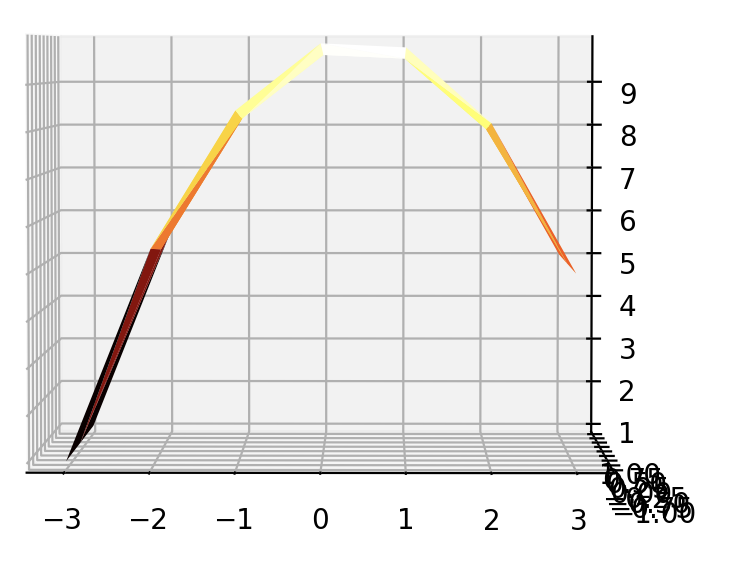
\includegraphics[width=\linewidth]{Materials/lowresc1}
		\caption{Low resolution mesh with curvature condition $c(p) = 1$.}
		\label{lowresc1}
	\end{subfigure}
	\hfill
	\begin{subfigure}[b]{0.49\linewidth}
		\centering
		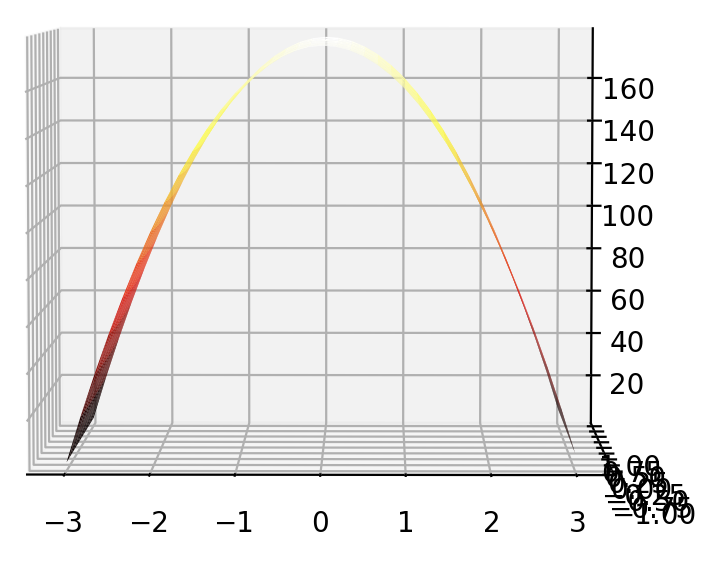
\includegraphics[width=\linewidth]{Materials/highresc1}
		\caption{High resolution mesh with curvature condition $c(p) = 1$.}
		\label{highresc1}
	\end{subfigure}
	\caption{Low and high resolution meshes with curvature condition $c(p) = 1$.}
	\label{c1meshes}
\end{figure}
We here note the much more jagged shaped of \autoref{lowresc1} compared to the very smooth shape of \autoref{highresc1}. We also note that both meshes are defined over the same domain, but the arc of \autoref{highresc1} goes much higher up than  \autoref{lowresc1}.  We can now take a look at the same mesh resolutions but with $c(p) = 0$. The results are shown in \autoref{c0meshes}.
\begin{figure}[H]
	\centering
	\begin{subfigure}[b]{0.49\linewidth}
		\centering
		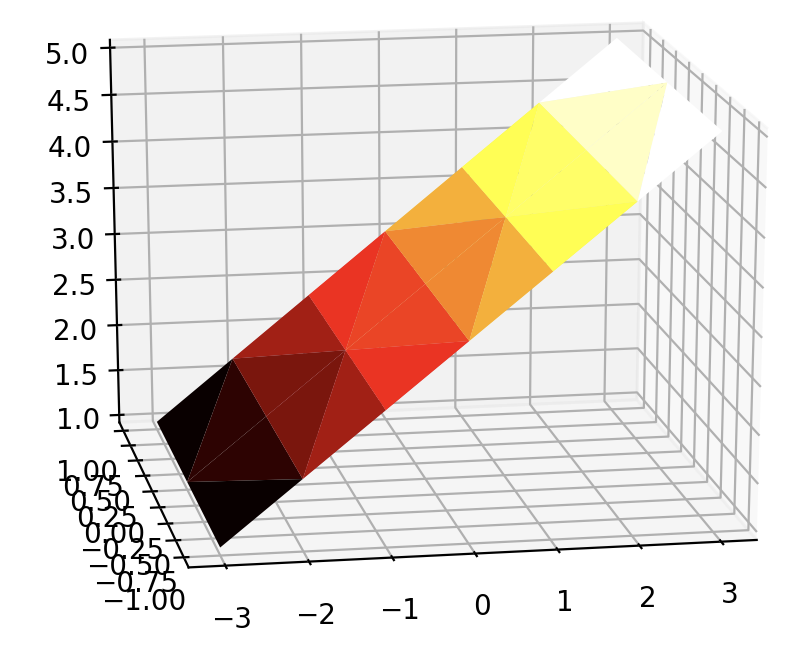
\includegraphics[width=\linewidth]{Materials/lowresc0}
		\caption{Low resolution mesh with curvature condition $c(p) = 0$.}
		\label{lowresc0}
	\end{subfigure}
	\hfill
	\begin{subfigure}[b]{0.49\linewidth}
		\centering
		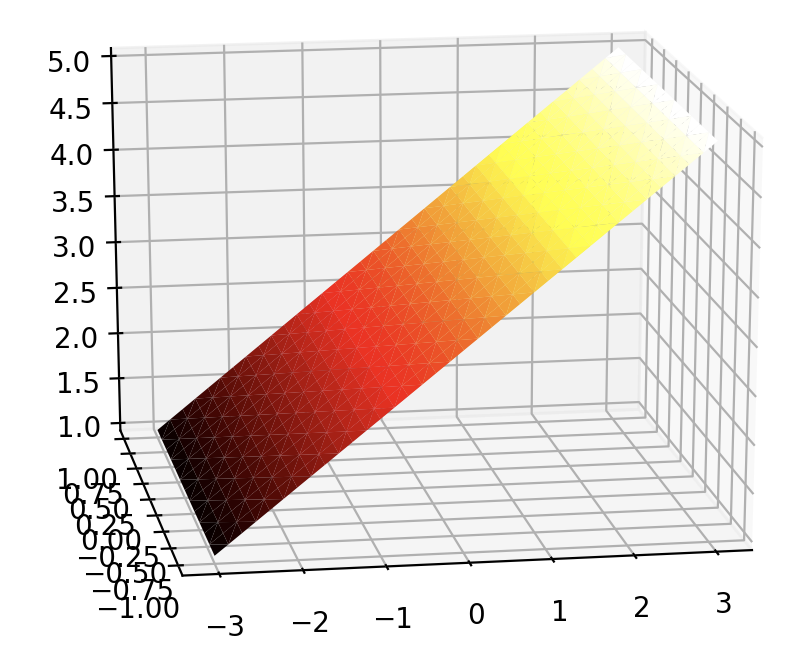
\includegraphics[width=\linewidth]{Materials/highresc0}
		\caption{High resolution mesh with curvature condition $c(p) = 0$.}
		\label{highresc0}
	\end{subfigure}
	\caption{Low and high resolution meshes with curvature condition $c(p) = 0$.}
	\label{c0meshes}
\end{figure}
Rather unsurprisingly we here see two solutions which looks very much the same. They both go completely linearly from the first to the second boundary condition. However, we do note we have a lot more nodes in the high resolution mesh, which means this is a much better approximation to the unknown function.

\subsubsection{Discussion of results}
From \autoref{lowresc0} and \autoref{highresc0} we see that our results matches our expectations as increasing the resolution simply gives us the same solution but with more nodes in the mesh and thus a better approximation. However, the same is not true for \autoref{lowresc1} and \autoref{highresc1}. We here see that when we have a fixed curvature for all elements, the curvature condition will apply between all nodes and thus get applied a lot more on high resolution meshes. This is why the arc in \autoref{highresc1} goes a lot higher than the arc in \autoref{lowresc1}. As we now understand that the number of nodes in the mesh influences the curvature of the mesh we could try to divide the wanted curvature by the number of nodes in the mesh. The results can be seen in \autoref{normalizedcurvature}.
\begin{figure}[H]
	\centering
	\begin{subfigure}[b]{0.49\linewidth}
		\centering
		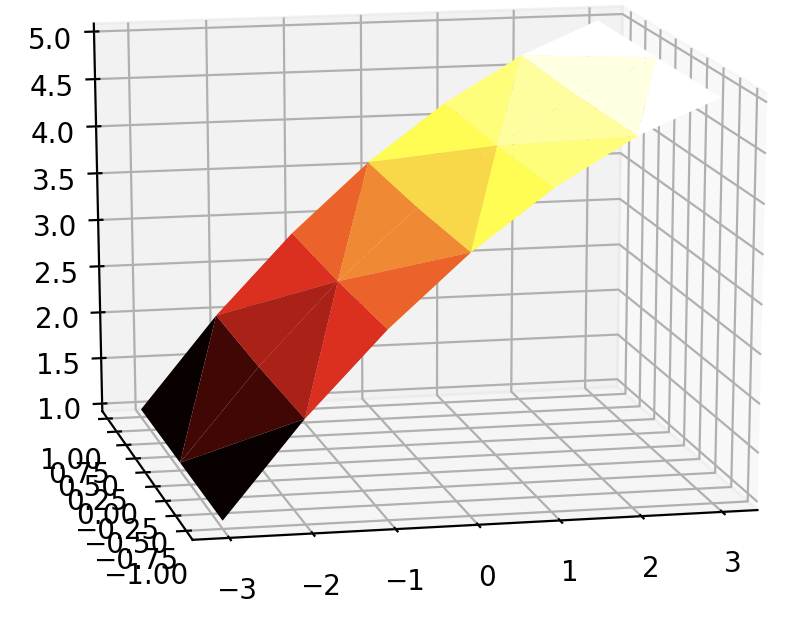
\includegraphics[width=\linewidth]{Materials/lownormal}
		\caption{Low resolution mesh with curvature condition $c(p) = 1 / (6\cdot 2)$.}
		\label{lownormal}
	\end{subfigure}
	\hfill
	\begin{subfigure}[b]{0.49\linewidth}
		\centering
		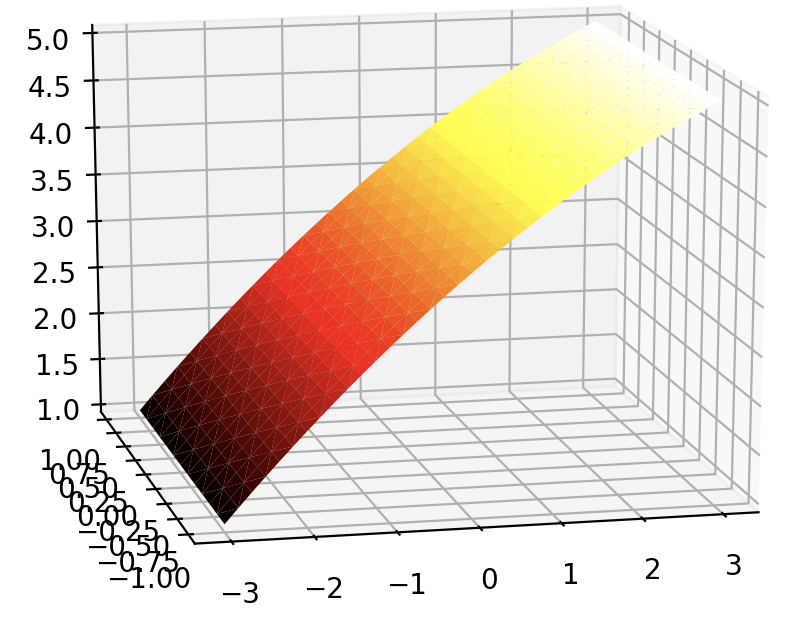
\includegraphics[width=\linewidth]{Materials/highnormal}
		\caption{High resolution mesh with curvature condition $c(p) = 1 / (36\cdot 12)$.}
		\label{highnormal}
	\end{subfigure}
	\caption{Results of normalizing the fixed curvature by the number of nodes in the mesh.}
	\label{normalizedcurvature}
\end{figure}
We now see very similar results as to \autoref{lowresc0} and \autoref{highresc0} where both meshes looks very much the same, and both meshes goes from the lower boundary to the upper boundary, but \autoref{highnormal} has a lot more nodes than \autoref{lownormal}. We thus conclude that increasing the mesh resolution greatly increases approximation accuracy, but if we have a curvature condition we will need to normalize it by the number of nodes in our mesh as our curvature condition is applied to all elements in the mesh.